\documentclass[a4paper,10pt]{article}
\usepackage[utf8]{inputenc}
\usepackage[final]{pdfpages}
\usepackage{caption}

\newcommand{\fw}{\linewidth}

\title{Math 660: Problem Set 4}
\author{Matthew Grasinger}

\begin{document}
  \maketitle

	\section{C1: Crank-Nicolson Scheme, Hyperbolic equations}
	

    {
      \centering
      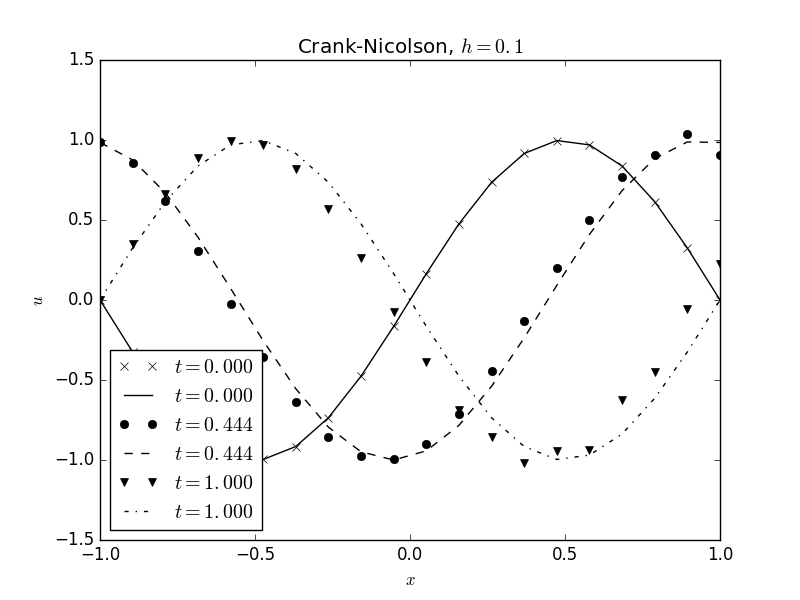
\includegraphics[width=\fw]{cn_thomas_M-20}
      \captionof{figure}{Crank-Nicolson scheme applied to the hyperbolic equation $u_t + u_x = 0$. The discretization is such that $h = \frac{1}{10}$ and $\lambda = 1.0$. The discrete solution (given by markers) is plotted with the exact solution (given by lines) for three different snapshots in time.}
      \vspace{0.25in}
      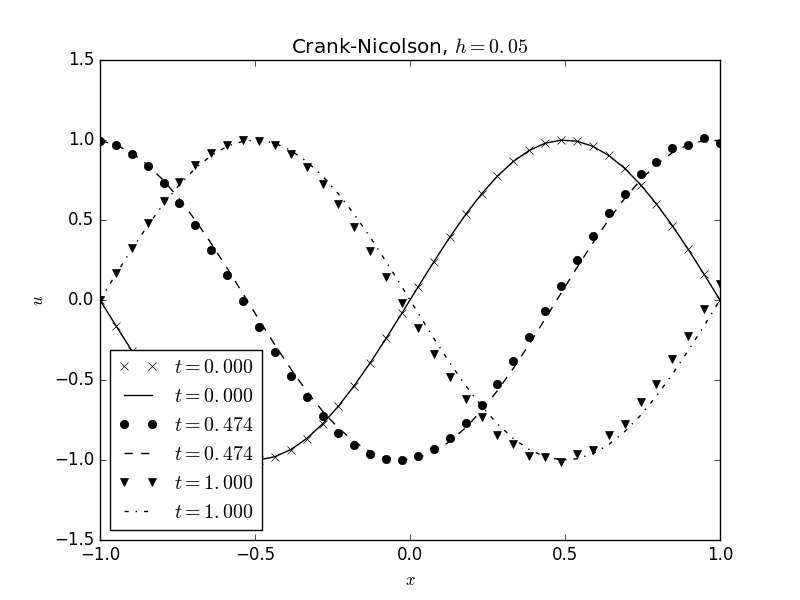
\includegraphics[width=\fw]{cn_thomas_M-40}
      \captionof{figure}{Crank-Nicolson scheme applied to the hyperbolic equation $u_t + u_x = 0$. The discretization is such that $h = \frac{1}{20}$ and $\lambda = 1.0$. The discrete solution (given by markers) is plotted with the exact solution (given by lines) for three different snapshots in time.}
      \vspace{0.25in}
      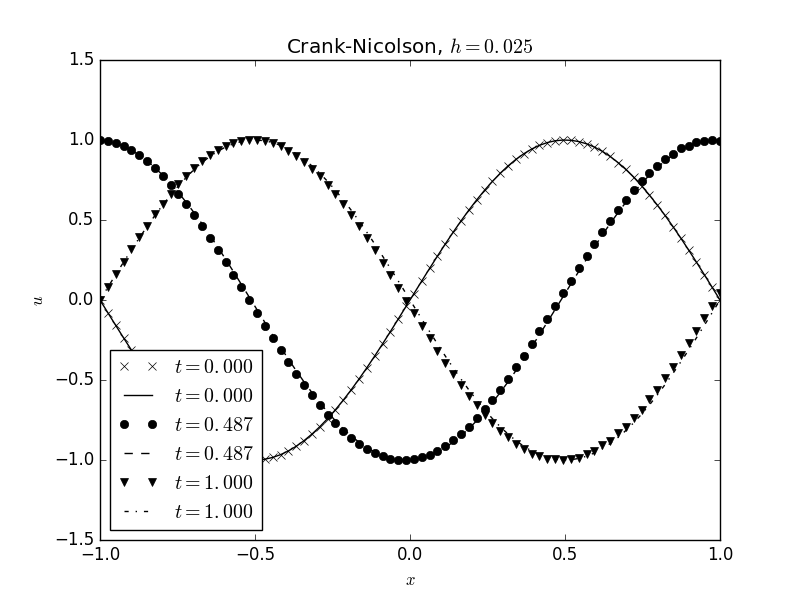
\includegraphics[width=\fw]{cn_thomas_M-80}
      \captionof{figure}{Crank-Nicolson scheme applied to the hyperbolic equation $u_t + u_x = 0$. The discretization is such that $h = \frac{1}{40}$ and $\lambda = 1.0$. The discrete solution (given by markers) is plotted with the exact solution (given by lines) for three different snapshots in time.}
      \vspace{0.25in}
    }
		
	\subsection{Source Code}
	
	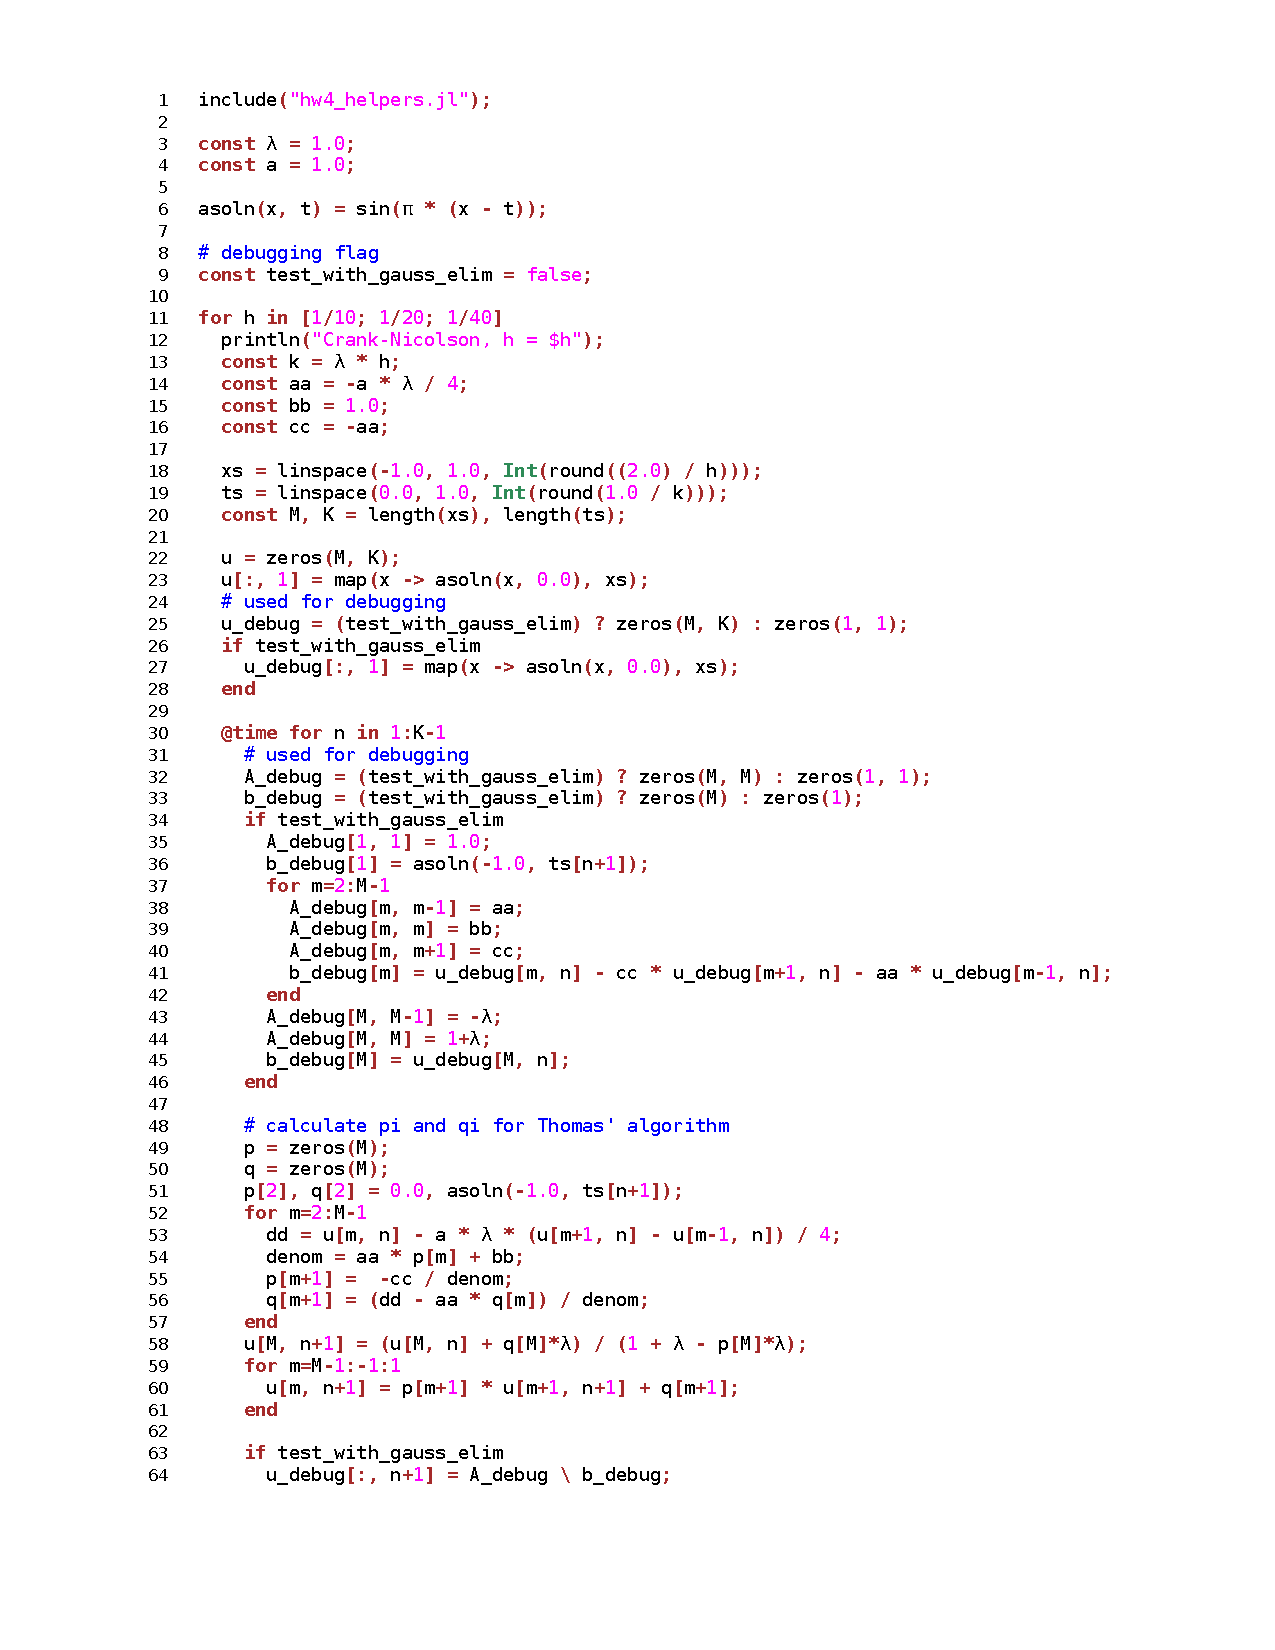
\includepdf[pages=-]{./hw4c1.pdf}
	
\end{document}
